\section{Results}
\label{sec:Auswertung}


\subsection{Laser threshold}

\begin{figure}
  \centering
  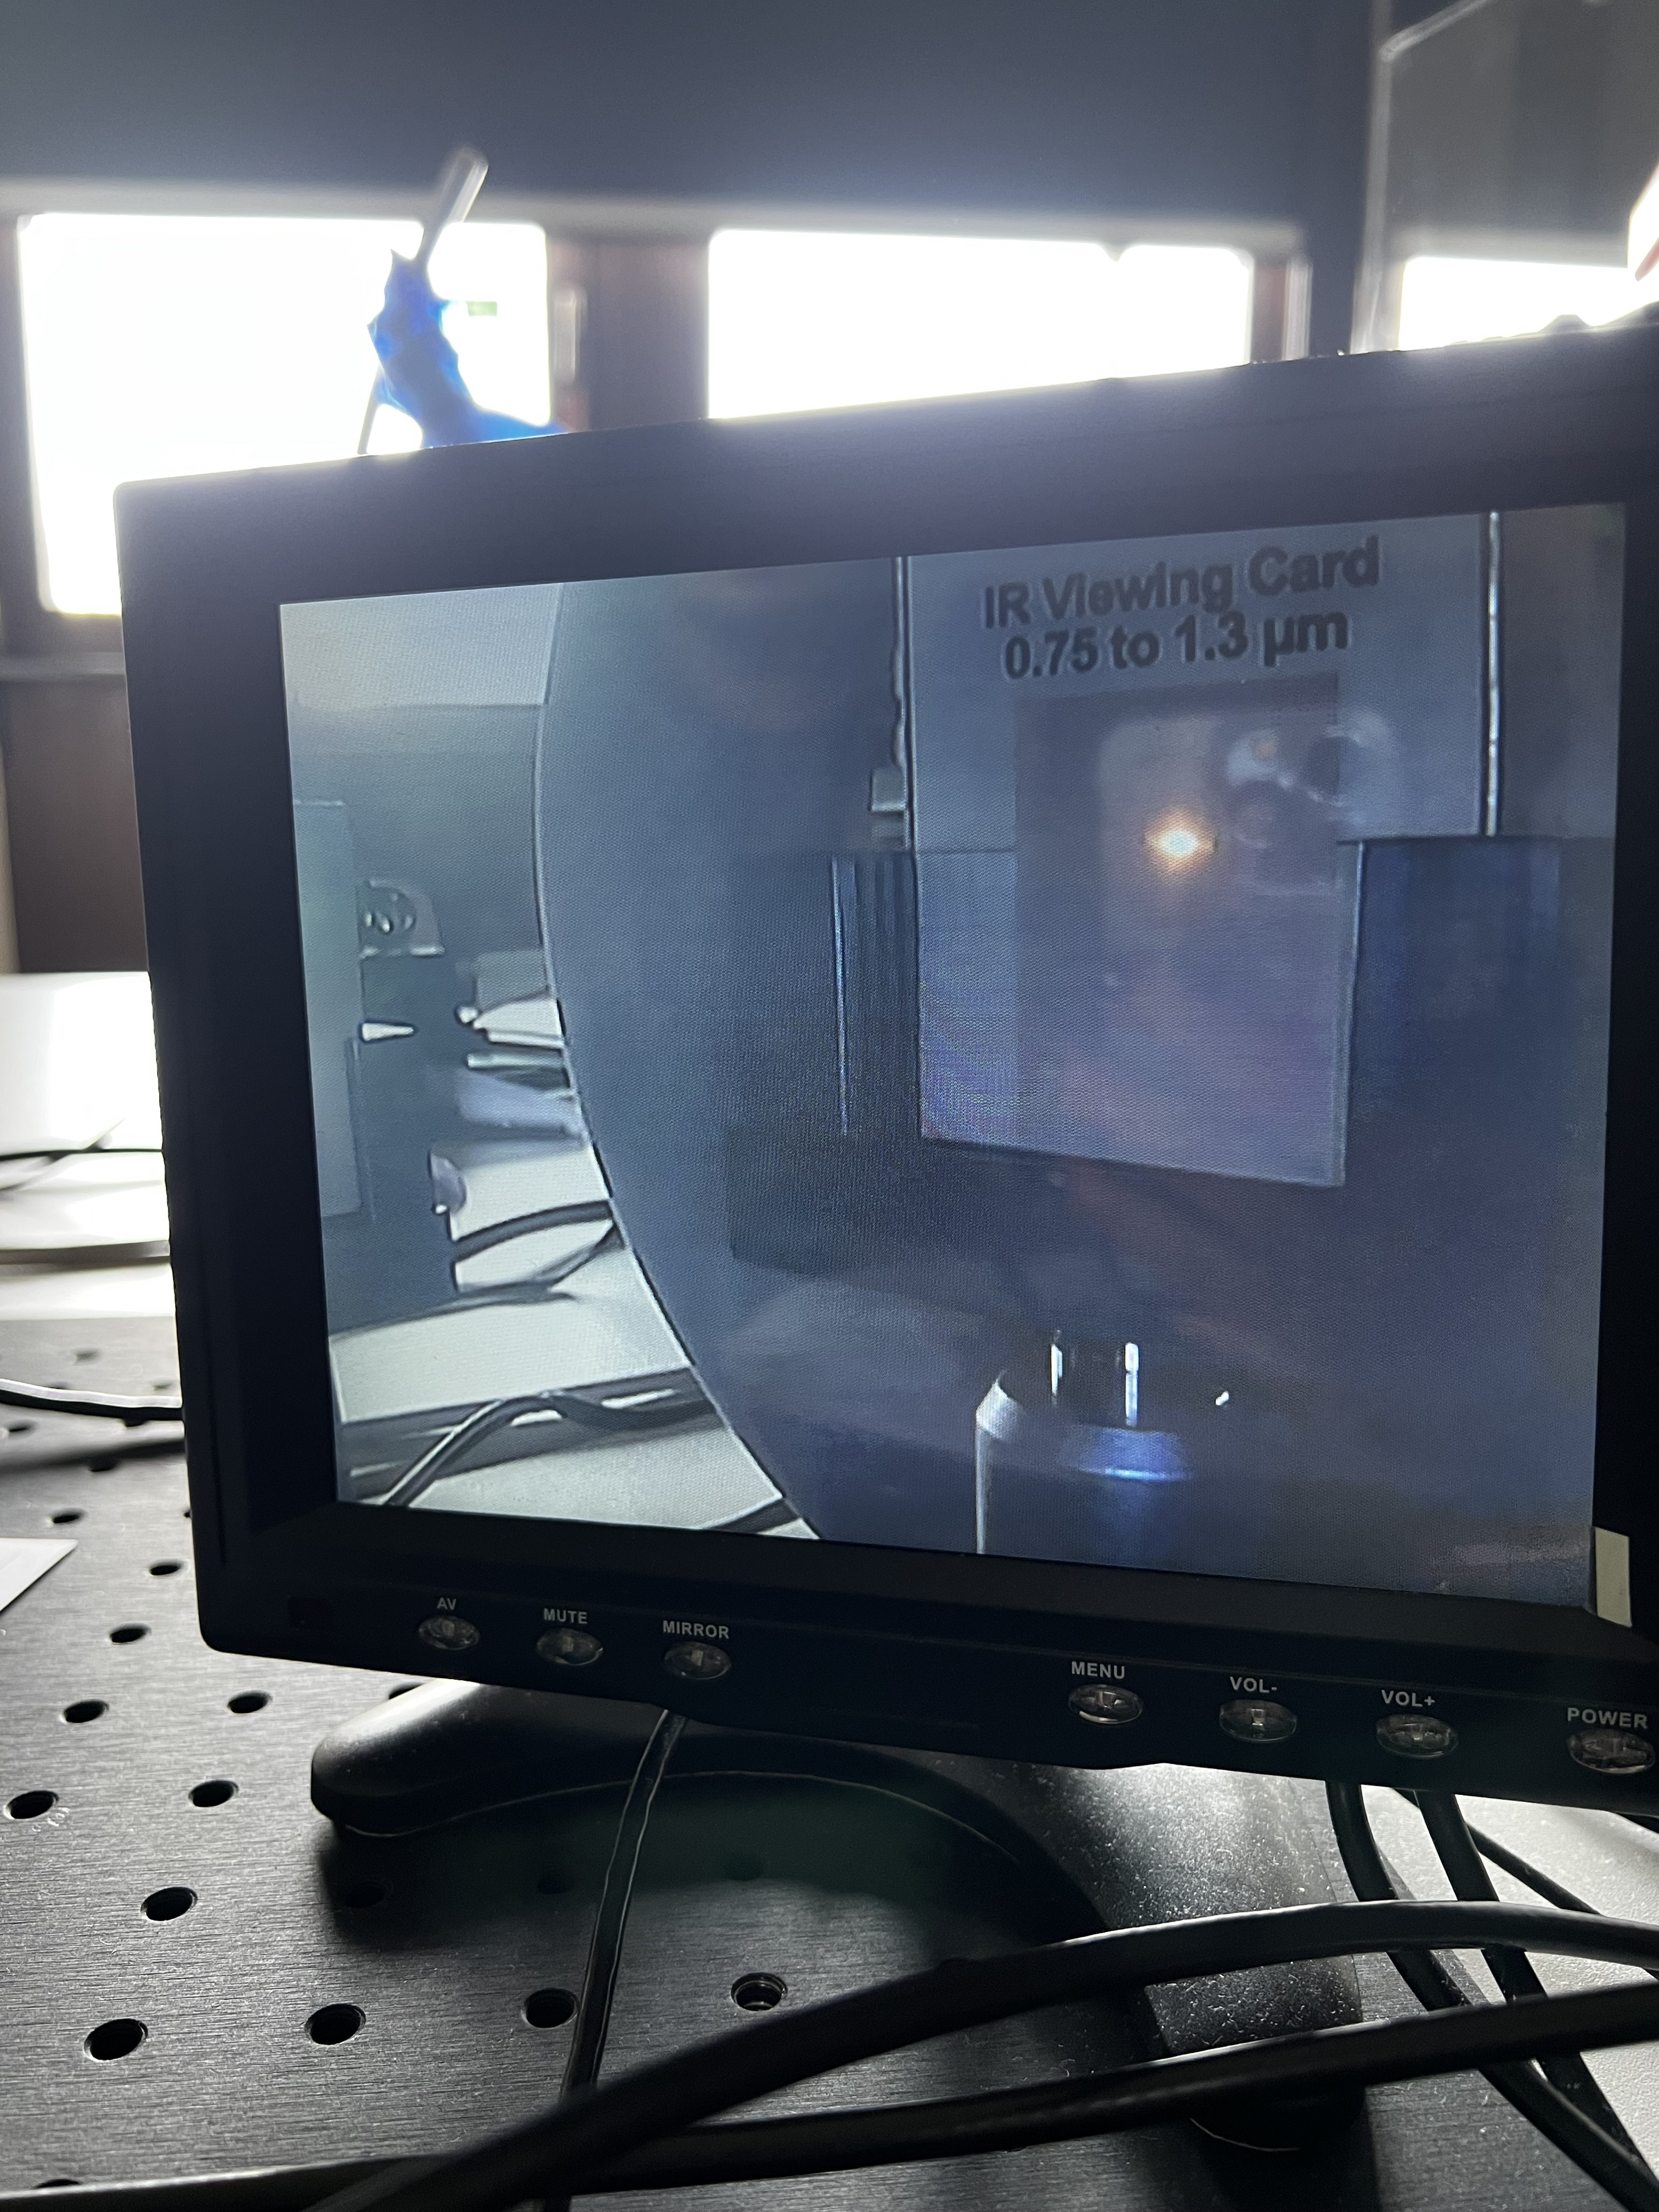
\includegraphics[width=0.5\textwidth]{content/LED.jpg}
  \caption{The current is below the threshold so the configuration is only an LED (Light-Emmitting Diode).}
  \label{fig:led}
\end{figure}

\begin{figure}
  \centering
  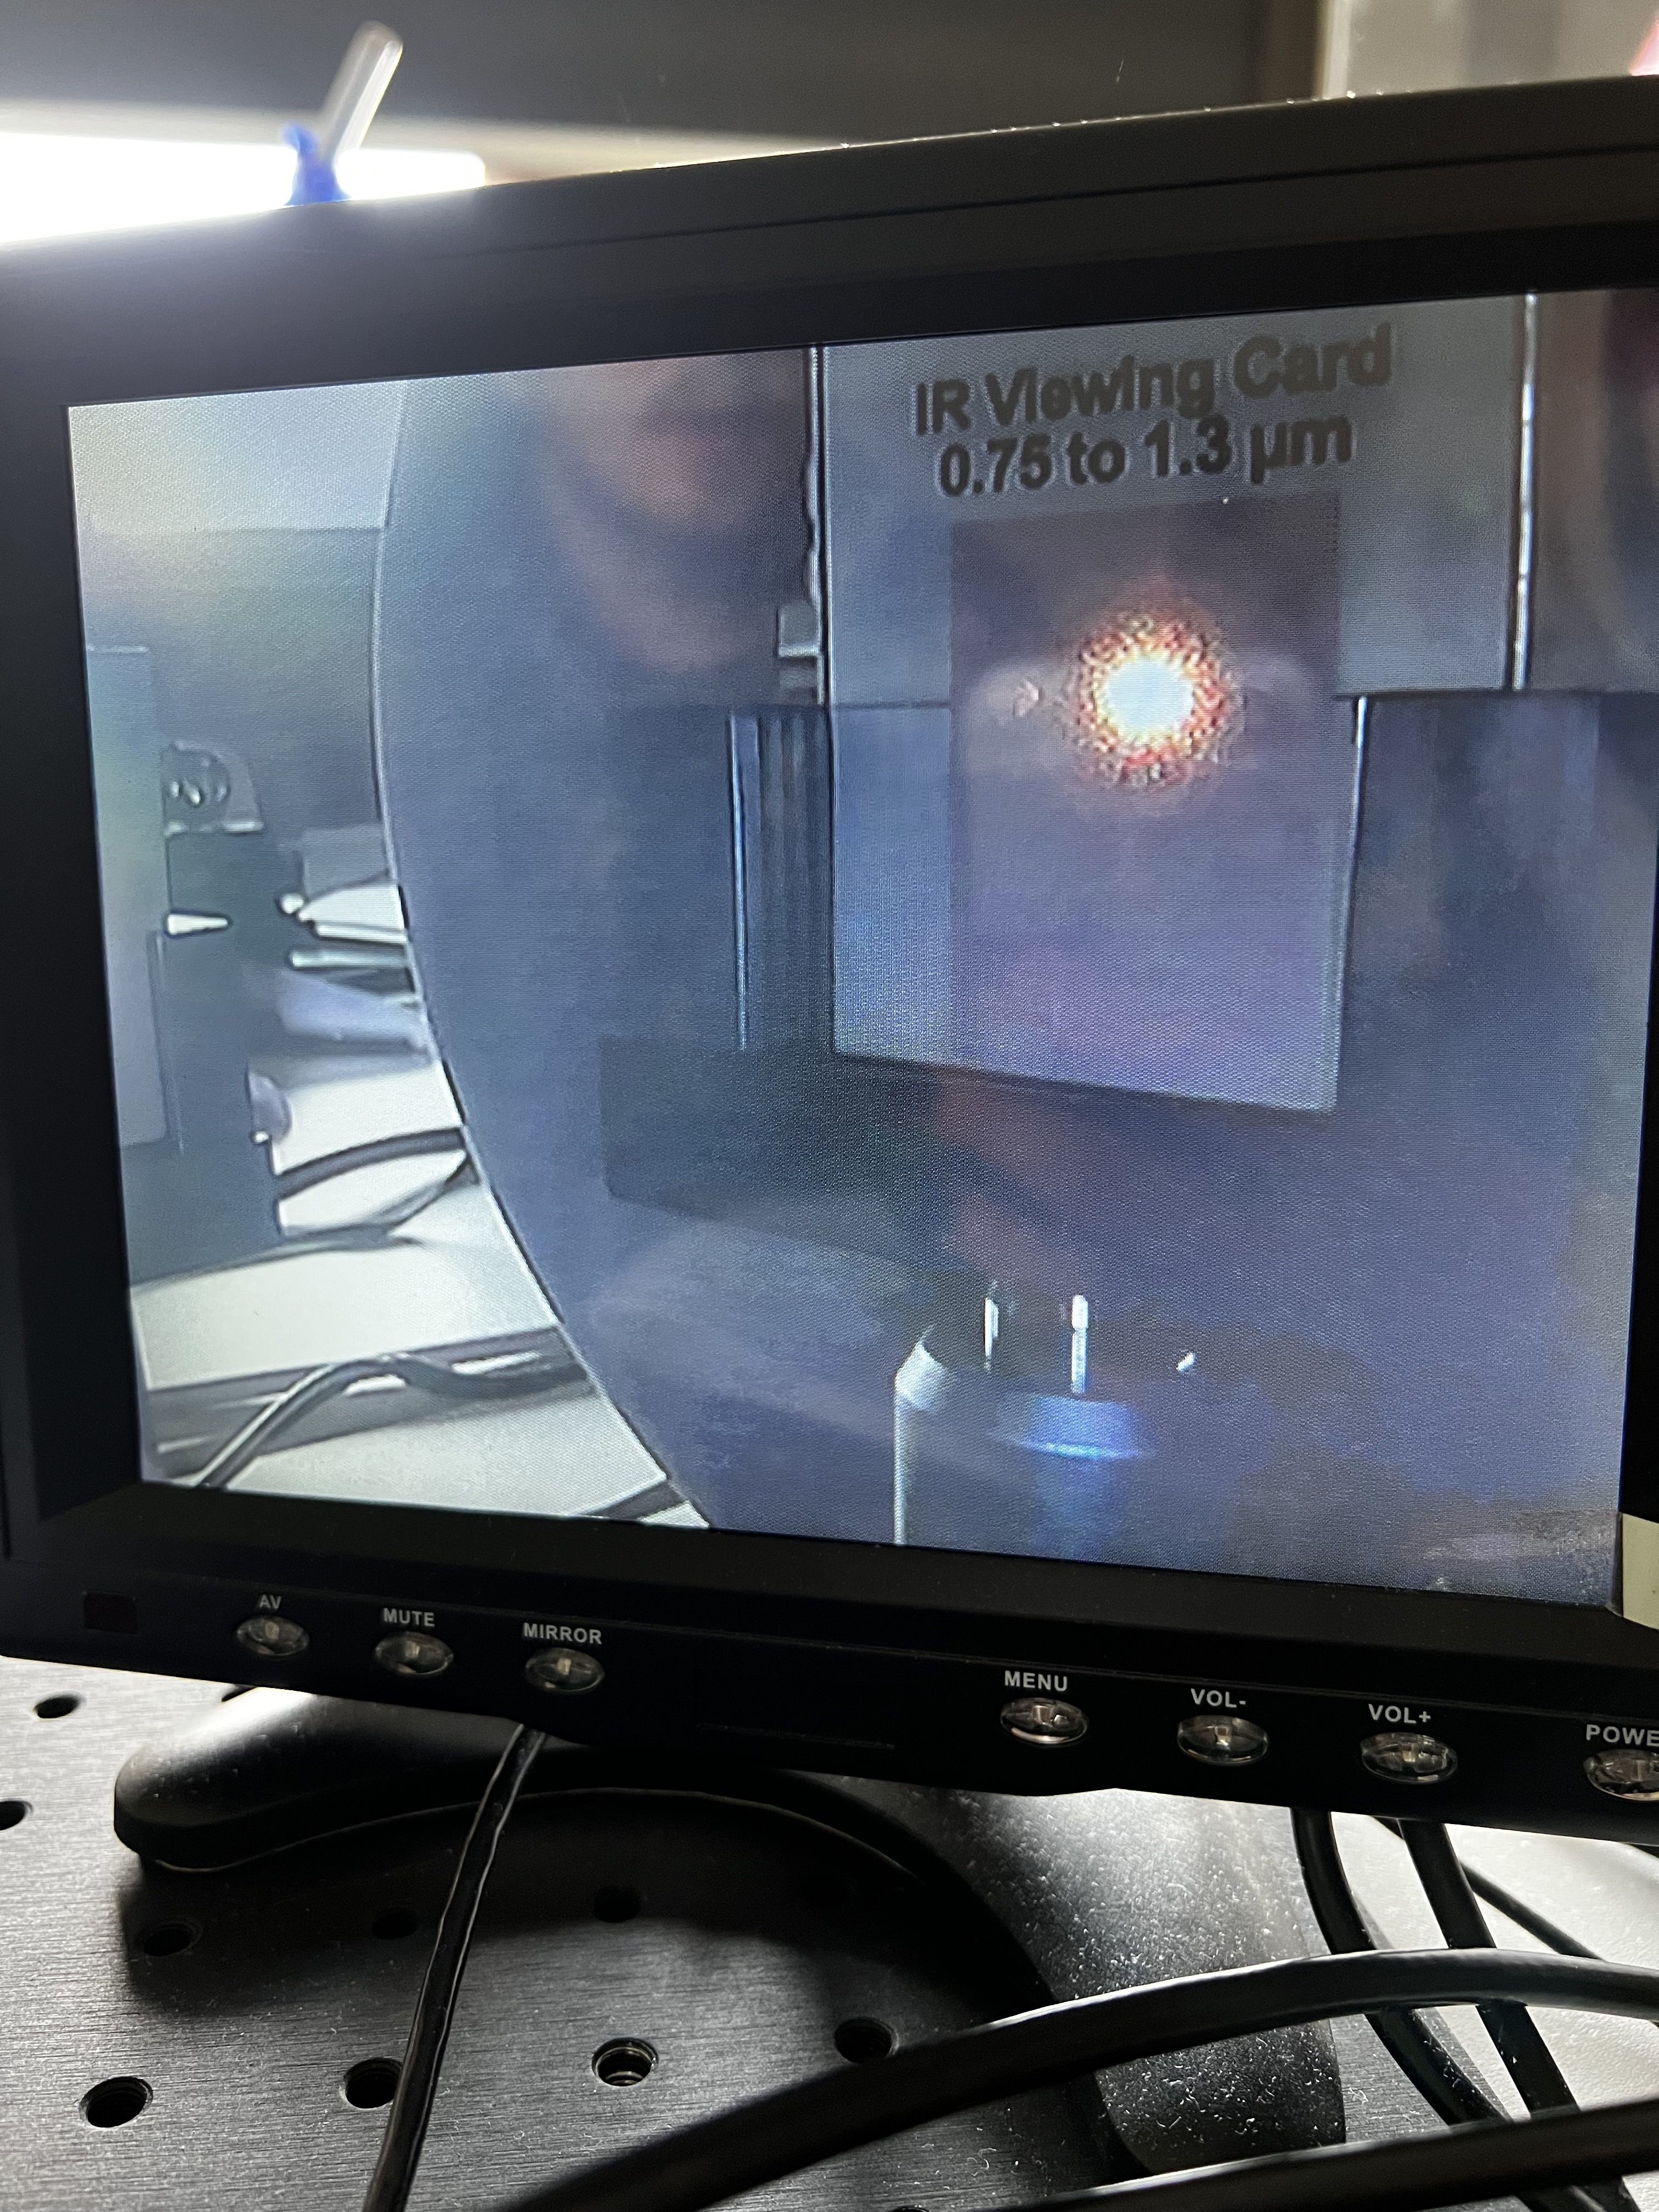
\includegraphics[width=0.5\textwidth]{content/laser.jpg}
  \caption{The current is set above the threshold value so that the charasterictic \grqq speckle\grqq{} of the laser beam is visible.}
  \label{fig:laser}
\end{figure}

The lasing threshold was measured to 36,7mA. Below this value the output is mainly produced by spontaneous emission and 
is smaller in size \autoref{fig:led} and not as bright as the laser beam \autoref{fig:laser}. \\
Also the laser beam is characterised by the granular \grqq speckle\grqq{} texture. 





\subsection{Rubidium fluorescence}

\begin{figure}
  \centering
  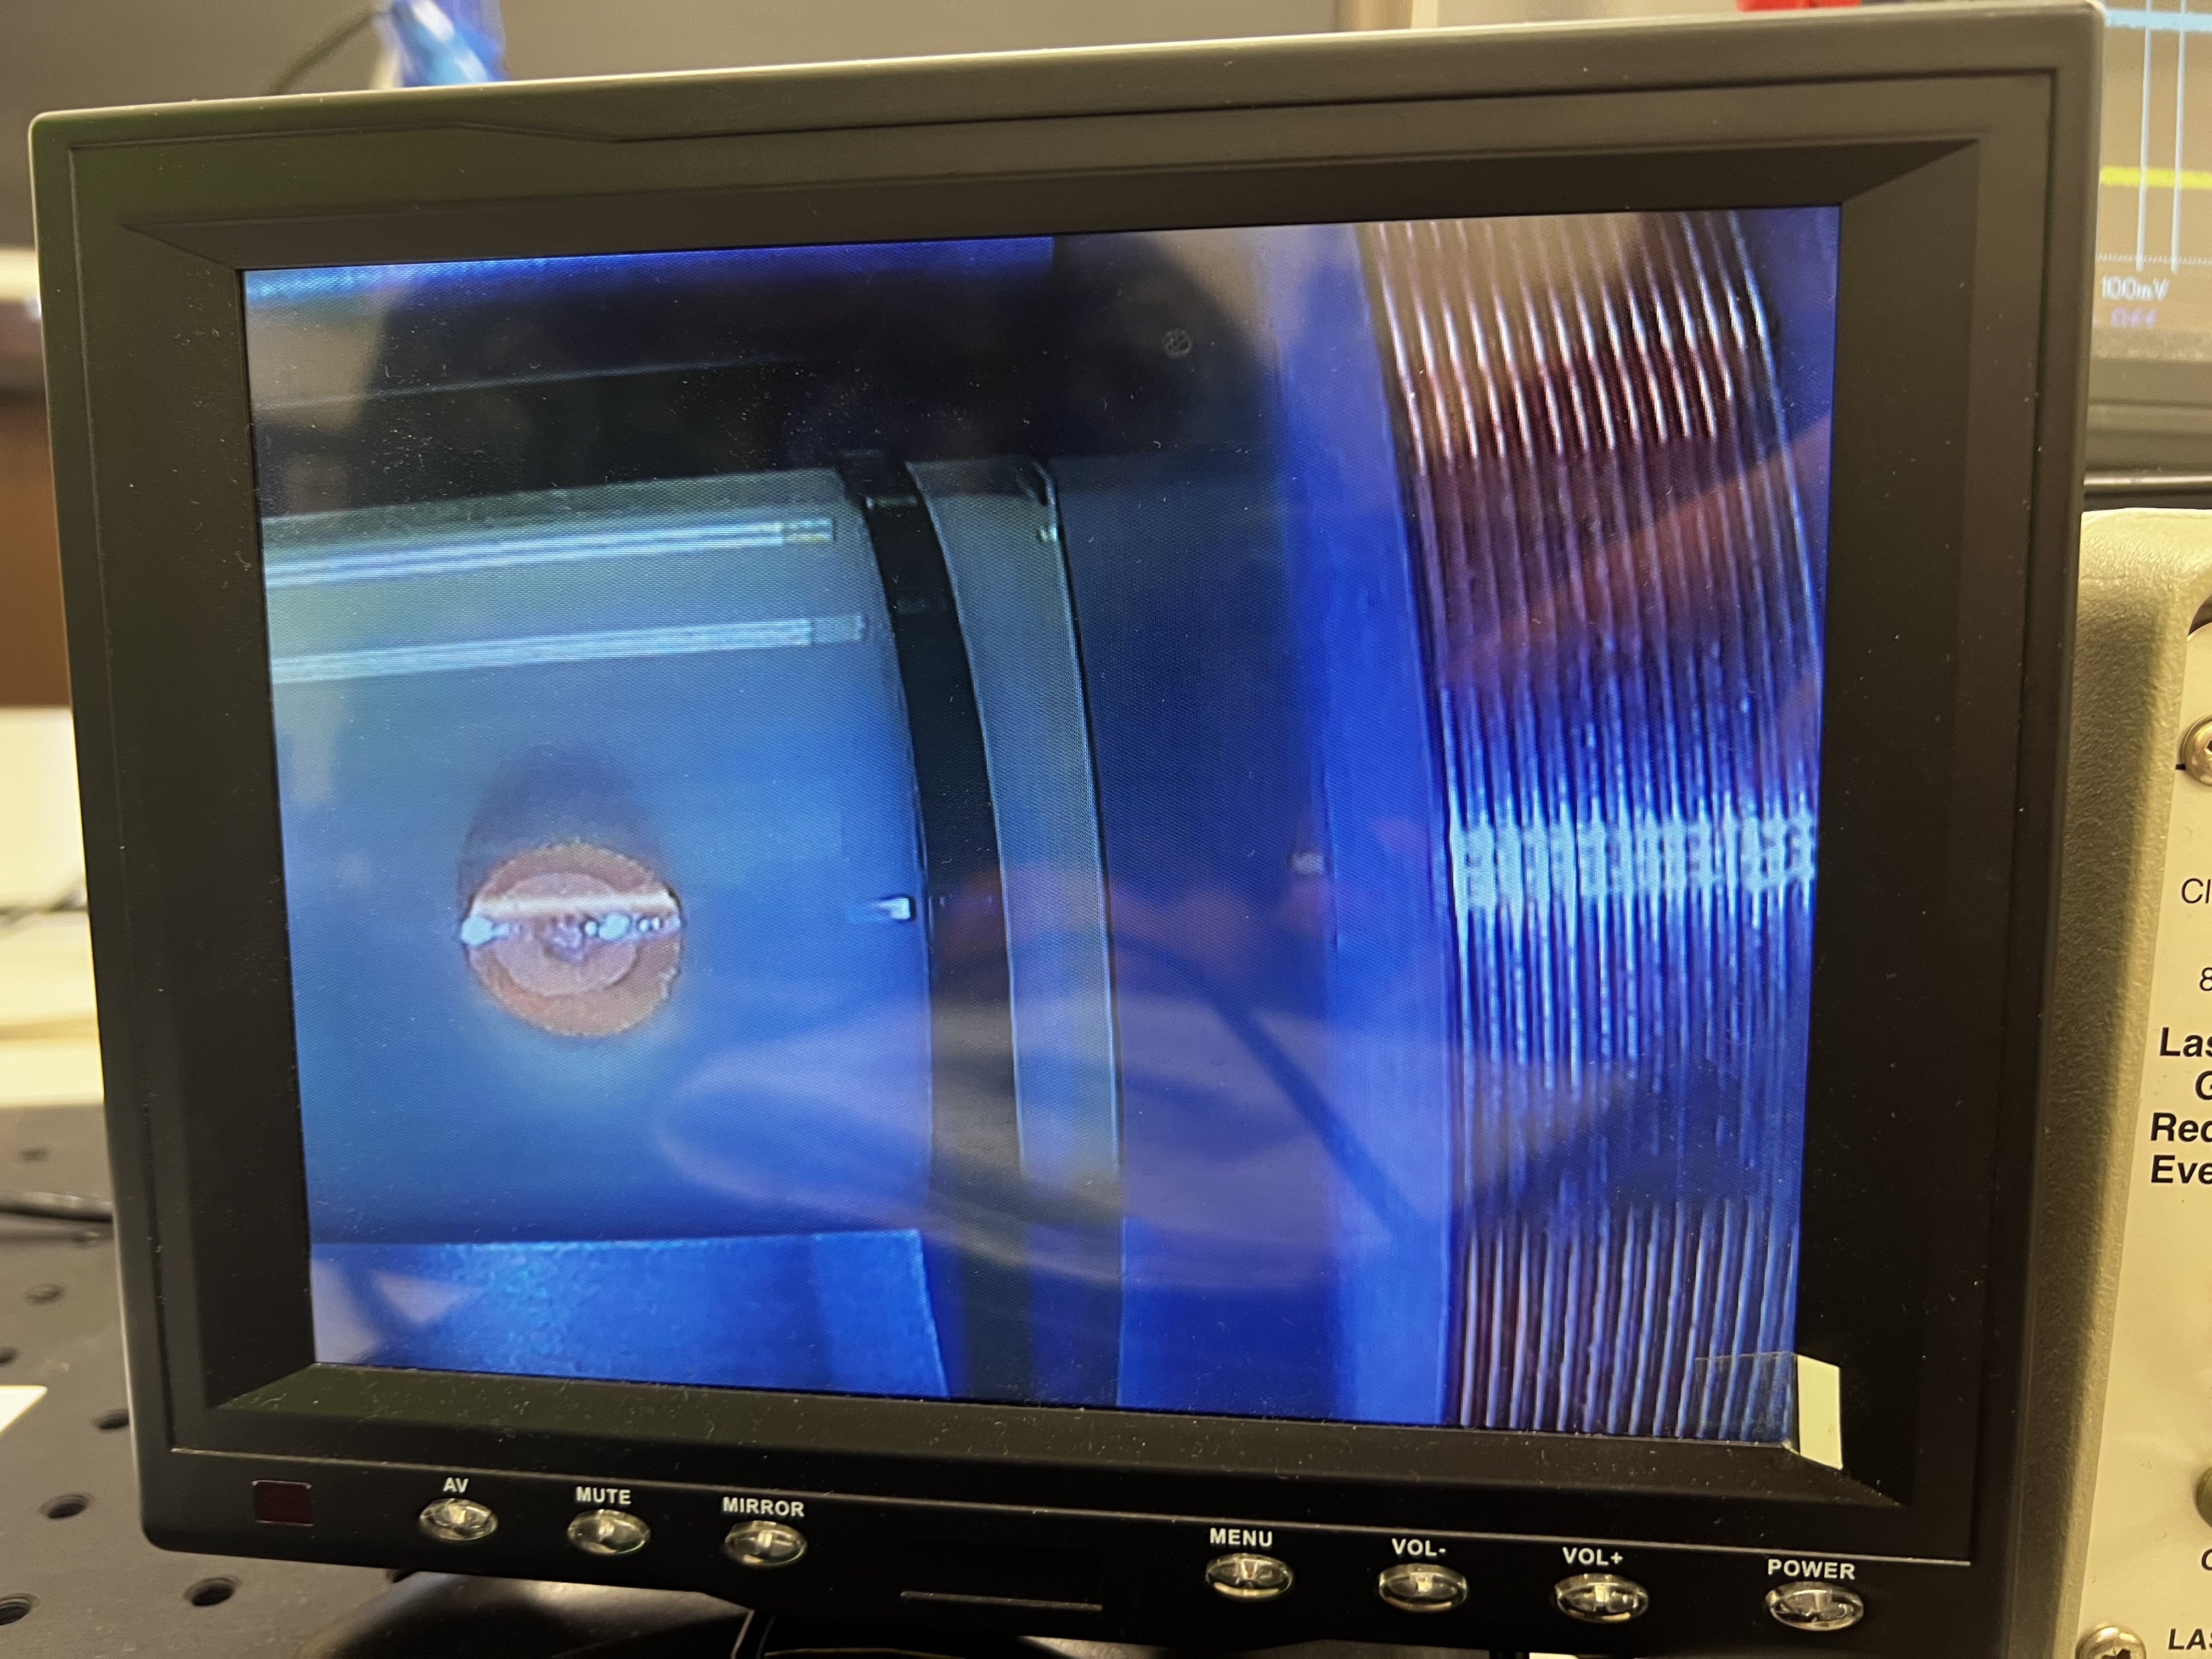
\includegraphics[width=0.5\textwidth]{content/horizontal.jpg}
  \caption{The Rubidium chamber is passed and excited by the laser beam which becomes visible.}
  \label{fig:horizontal}
\end{figure}

The side knob and thereby the wavelength of the laser is adjusted so that the laser beam is visible in the Rubidium chamber \autoref{fig:horizontal}.\\
When the laser beam passes the Rubidium gas it excites the Rubidium which is then emitting light by spontaneous emission. 








\subsection{Absorption spectrum of Rubidium}
\begin{figure}
  \centering
  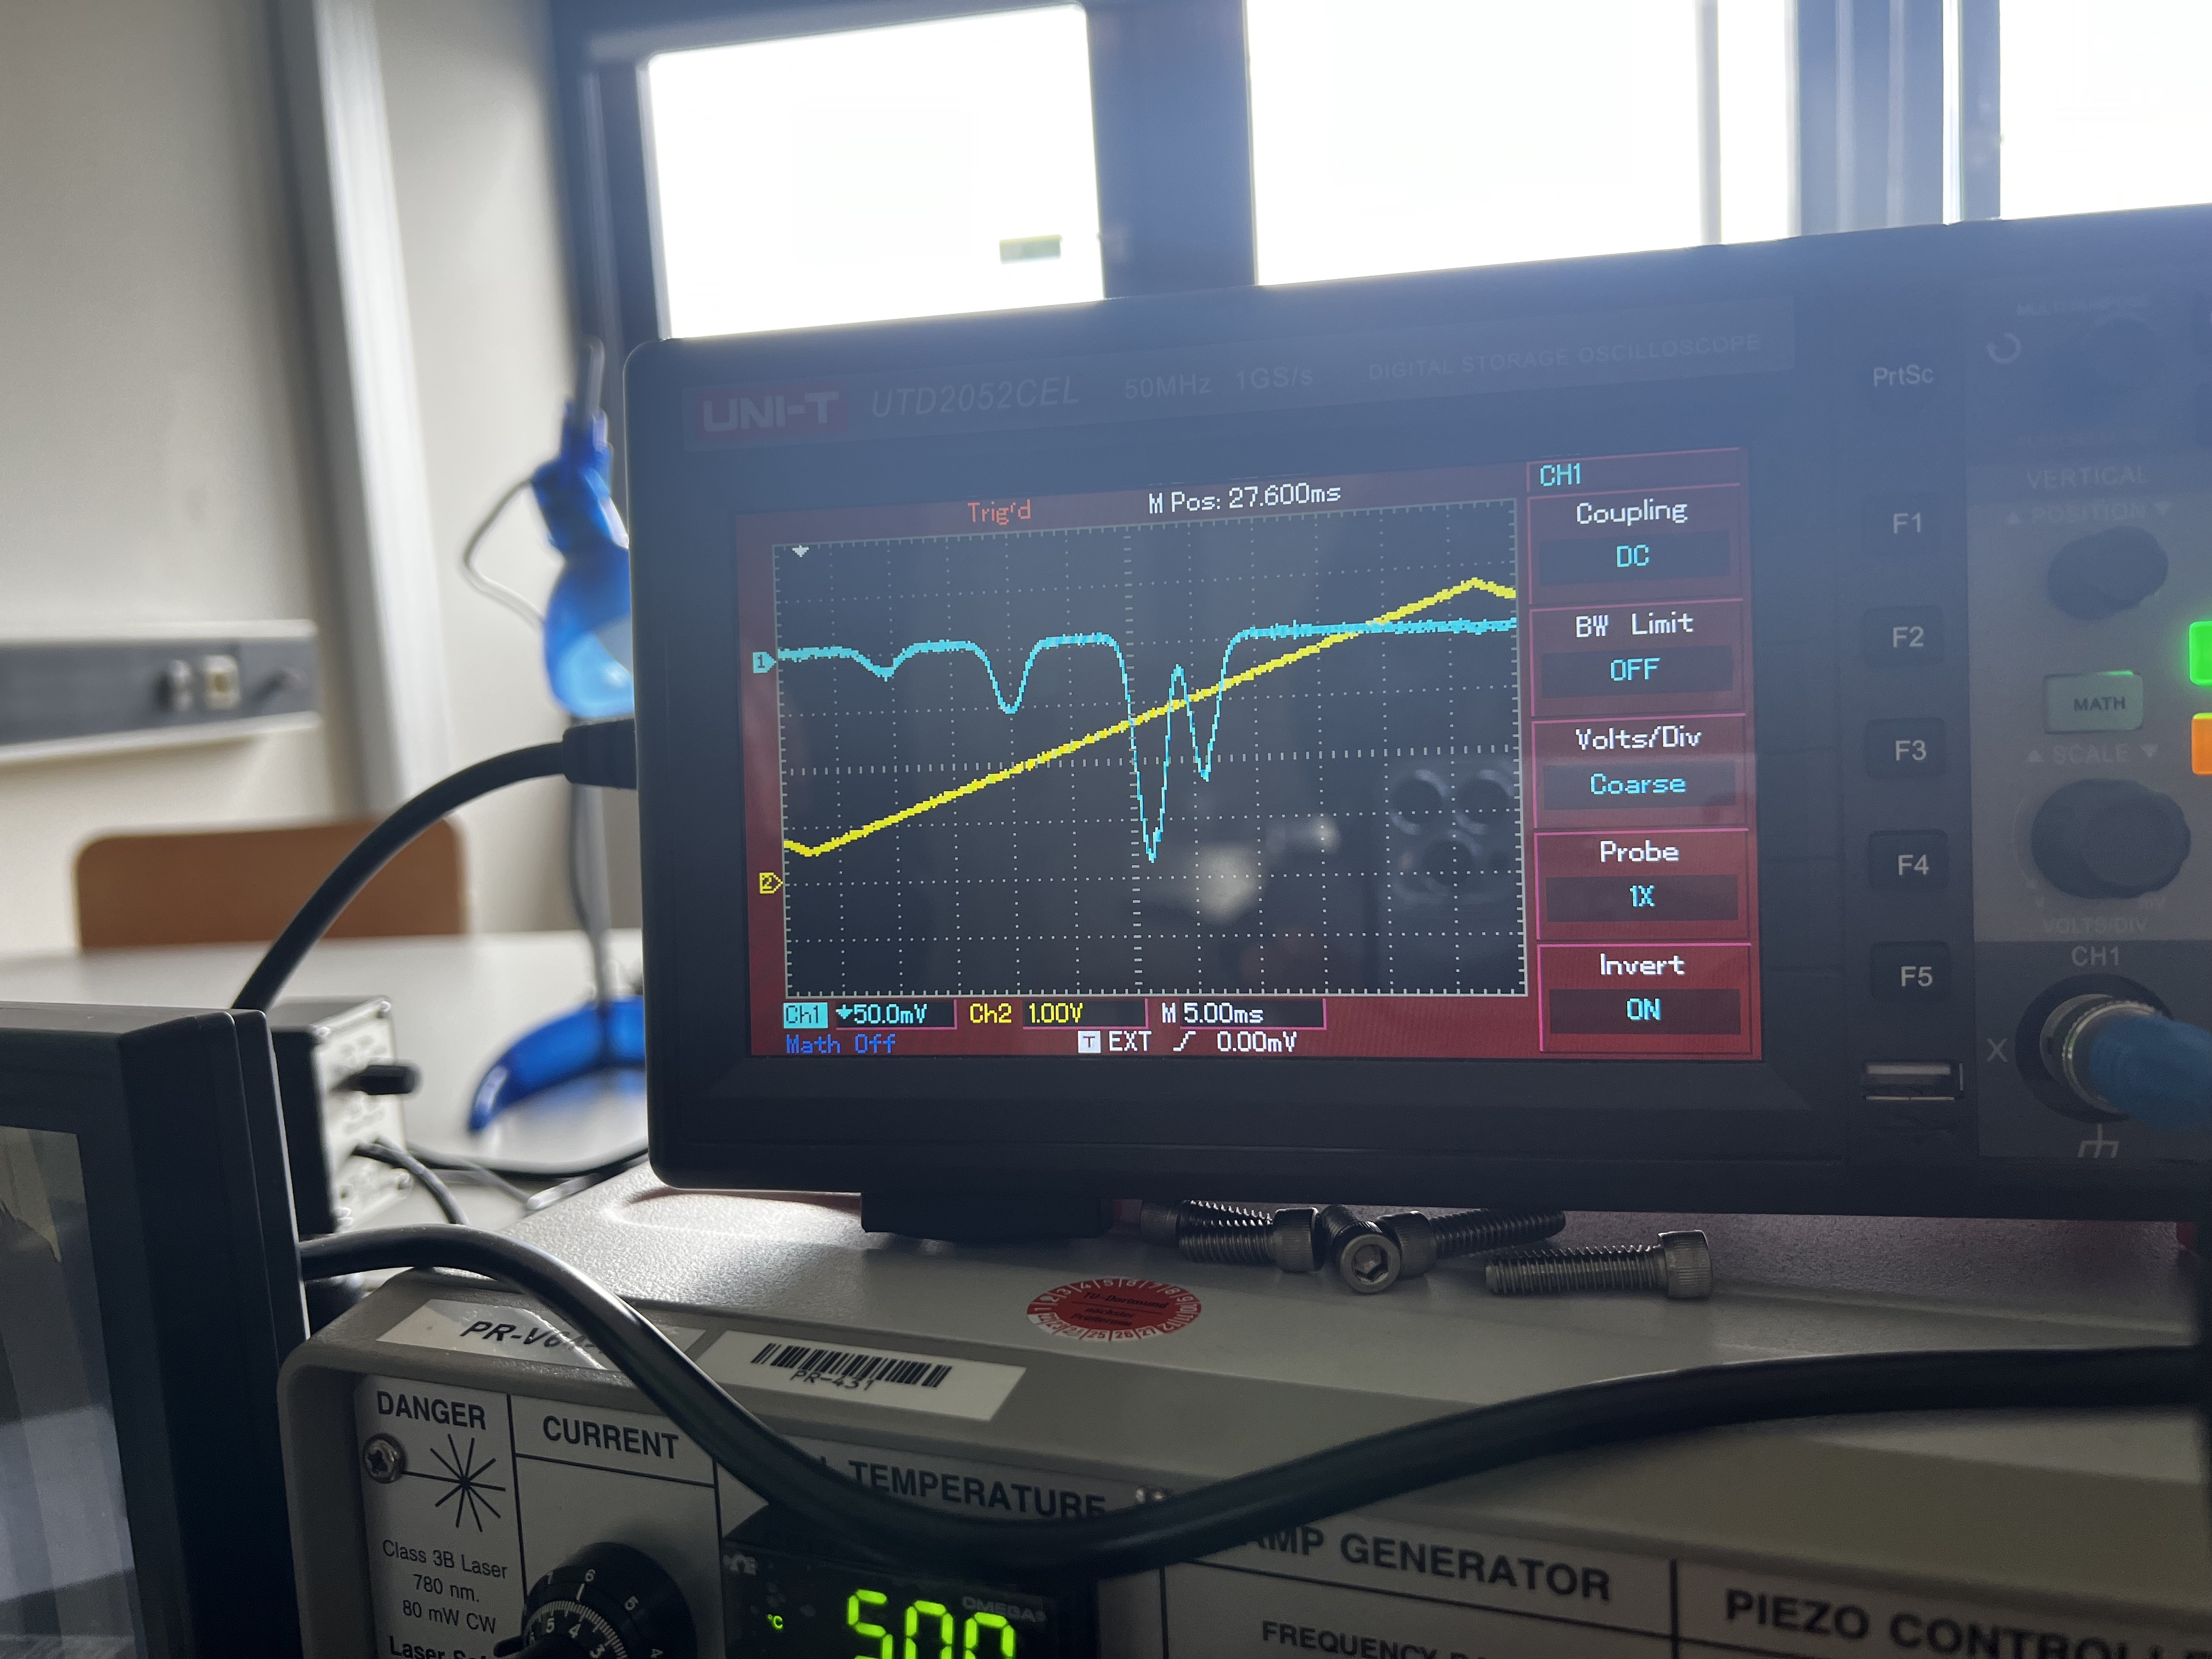
\includegraphics[width=0.5\textwidth]{content/absorption.jpg}
  \caption{The absorption spectrum of Rubidium and the triangular voltage applied to the piezoelectric stack.}
  \label{fig:absorption}
\end{figure}
The absorption spectrum is characterised by four peaks \autoref{fig:absorption}. Each one is caused by one of the four isotopes of Rubidium that 
are located in the Rubidium chamber. \\
The different magnitudes are explained by the uneven ratio of the isotopes. 

As certain voltage levels are applied to the piezo electric stack, it stimulates a change in energy level
and the absorption ratio of the Rubidium rises. This makes the curve symmetrical.





